%%%%%%%%%%%%%%%%%%%%%%%%%%%%%%%%%%%

\section{Examining the Central Limit Theorem}

%%%%%%%%%%%%%%%%%%%%%%%%%%%%%%%%%%%

\begin{frame}[fragile]
\frametitle{Average number of basketball games attended}

Next let's look at the population data for the number of basketball games attended:

\begin{center}
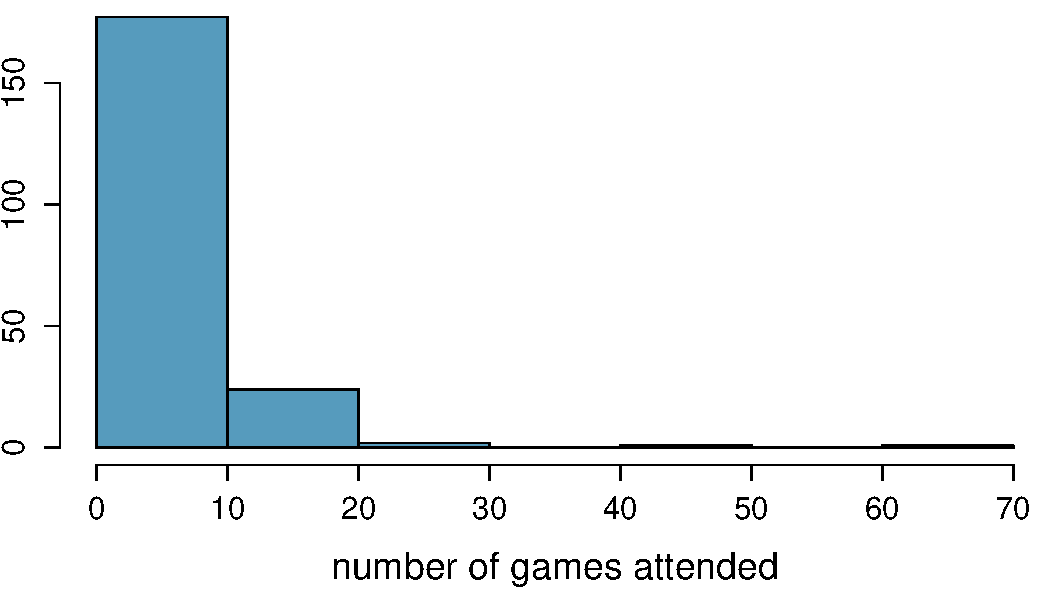
\includegraphics[width=0.8\textwidth]{4-4_clt/figures/duke_games/duke_games_pop}
\end{center}


\end{frame}


%%%%%%%%%%%%%%%%%%%%%%%%%%%%%%%%%%%

\begin{frame}[fragile]
\frametitle{Average number of basketball games attended (cont.)}

Sampling distribution, n = 10:

\twocol{0.6}{0.4}{
\begin{center}
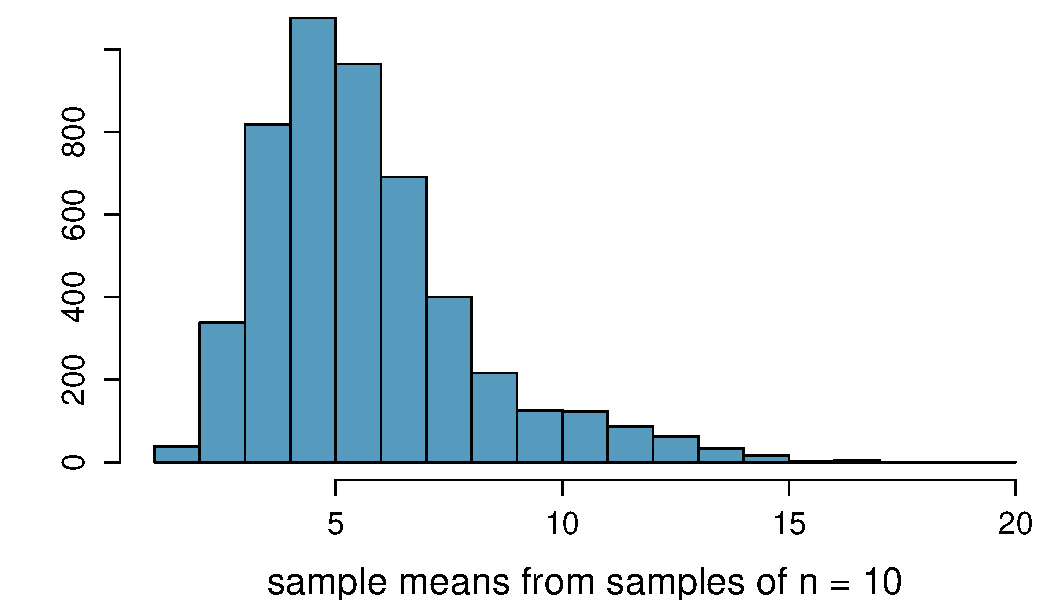
\includegraphics[width=\textwidth]{4-4_clt/figures/duke_games/duke_games_n10}
\end{center}
}
{
\dq{What does each observation in this distribution represent?}
\soln{\only<1>{\textcolor{white}{Sample mean ($\bar{x}$) of samples of size $n = 10$.}}}
\soln{\only<2->{Sample mean ($\bar{x}$) of samples of size $n = 10$.}}
\dq{Is the variability of the sampling distribution smaller or larger than the variability of the population distribution? Why?}
\soln{\only<1-2>{\textcolor{white}{Smaller, sample means will vary less than individual observations.}}}
\soln{\only<3->{Smaller, sample means will vary less than individual observations.}}
}

\end{frame}


%%%%%%%%%%%%%%%%%%%%%%%%%%%%%%%%%%%%

\begin{frame}[fragile]
\frametitle{Average number of basketball games attended (cont.)}

Sampling distribution, n = 30:

\twocol{0.6}{0.4}{
\begin{center}
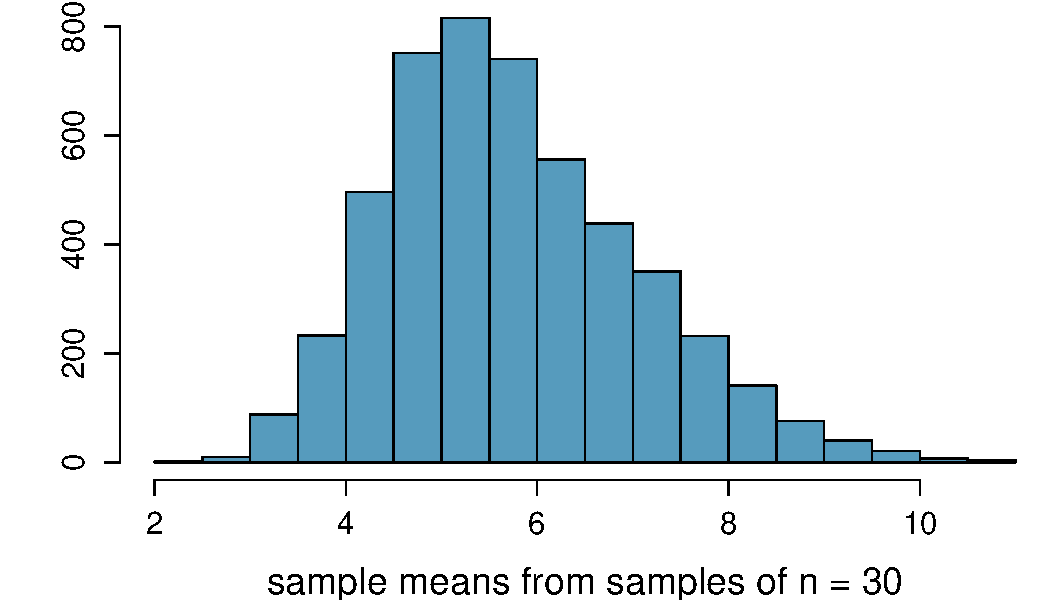
\includegraphics[width=\textwidth]{4-4_clt/figures/duke_games/duke_games_n30}
\end{center}
}
{
\dq{How did the shape, center, and spread of the sampling distribution change going from $n = 10$ to $n = 30$?}
\soln{\only<1>{\textcolor{white}{Shape is more symmetric, center is about the same, spread is smaller.}}}
\soln{\only<2->{Shape is more symmetric, center is about the same, spread is smaller.}}
}

\end{frame}


%%%%%%%%%%%%%%%%%%%%%%%%%%%%%%%%%%%%

\begin{frame}[fragile]
\frametitle{Average number of basketball games attended (cont.)}

Sampling distribution, n = 70:

\begin{center}
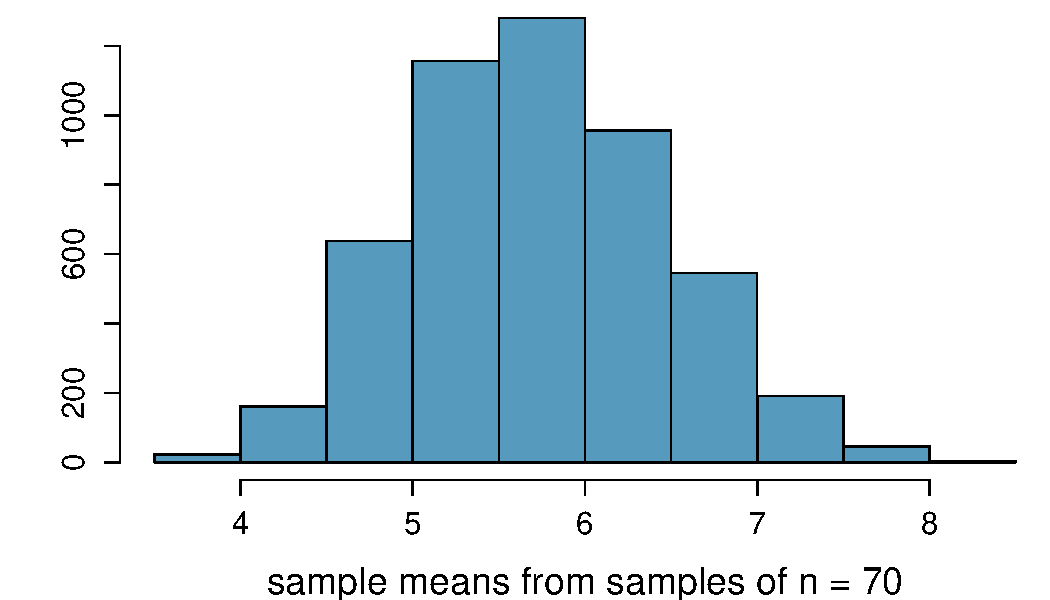
\includegraphics[width=0.6\textwidth]{4-4_clt/figures/duke_games/duke_games_n70}
\end{center}

\end{frame}


%%%%%%%%%%%%%%%%%%%%%%%%%%%%%%%%%%%%

\begin{frame}[fragile]
\frametitle{Average number of basketball games attended (cont.)}

\dq{The mean of the sampling distribution is 5.75, and the standard deviation of the sampling distribution (also called the \hl{standard error}) is 0.75. Which of the following is the most reasonable guess for the 95\% confidence interval for the true average number of basketball games attended by students?}

\begin{enumerate}[(a)]
\item $5.75 \pm 0.75$
\solnMult{$5.75 \pm 2 \times 0.75$} \soln{\only<2>{\red{$\rightarrow (4.25,7.25)$}}}
\item $5.75 \pm 3 \times 0.75$
\item cannot tell from the information given
\end{enumerate}


\end{frame}

%%%%%%%%%%%%%%%%%%%%%%%%%%%%%%%%%%%

\begin{frame}
\frametitle{}

\pq{
{\footnotesize Four plots: Determine which plot (A, B, or C) is which. \\
(1) At top: distribution for a population ($\mu = 10, \sigma = 7$), \\
(2) a single random sample of 100 observations from this population, \\
(3) a distribution of 100 sample means from random samples with size 7, and \\
(4) a distribution of 100 sample means from random samples with size 49.}}

\twocol{0.4}{0.6}{
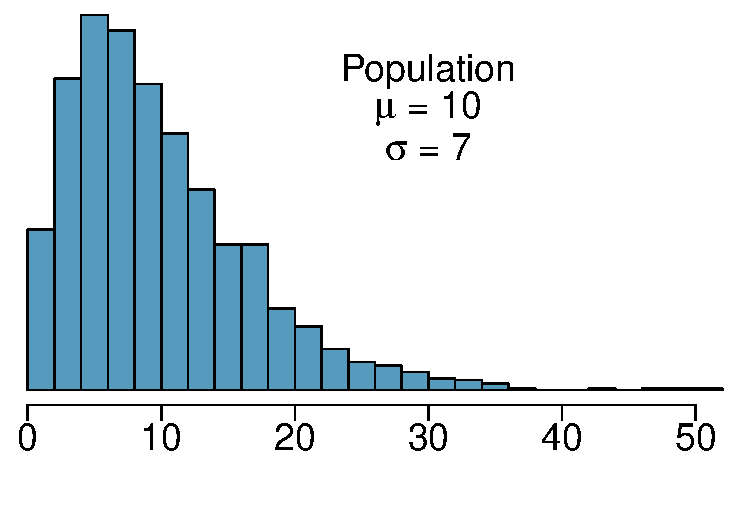
\includegraphics[width=\textwidth]{4-4_clt/figures/cltSimRS/cltSimRS_pop}
}
{
\vspace{-0.5cm}
{\small
\begin{enumerate}[(a)]
\solnMult{A - (3); B - (2); C - (4)}
\item A - (2); B - (3); C - (4)
\item A - (3); B - (4); C - (2)
\item A - (4); B - (2); C - (3)
\end{enumerate}
}
}
\vspace{-0.25cm}
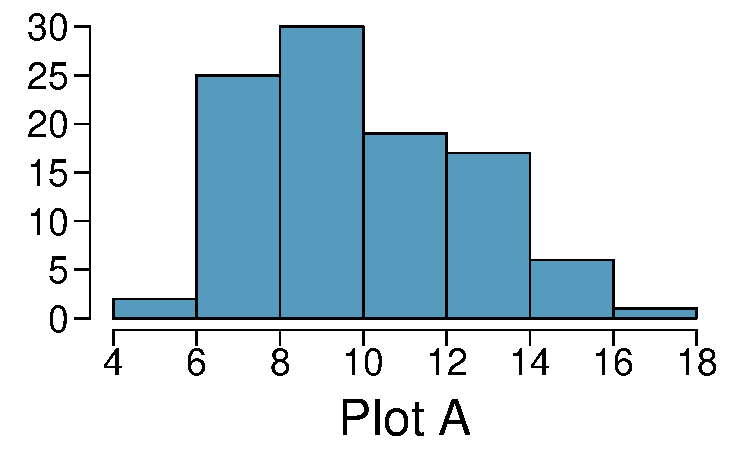
\includegraphics[width=0.32\textwidth]{4-4_clt/figures/cltSimRS/cltSimRS_n7}
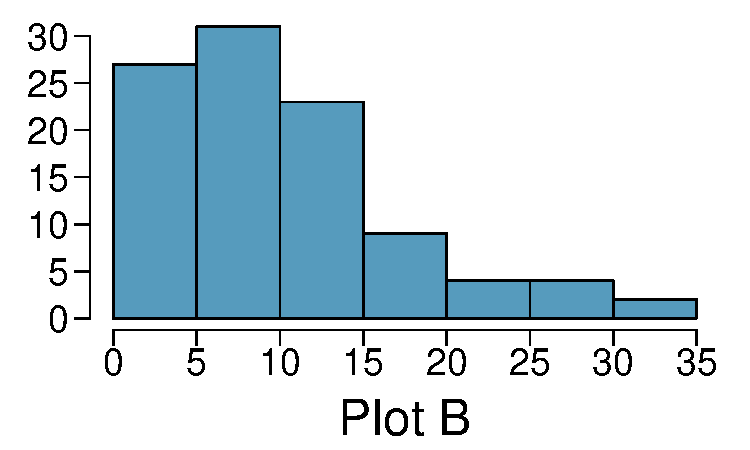
\includegraphics[width=0.32\textwidth]{4-4_clt/figures/cltSimRS/cltSimRS_samp}
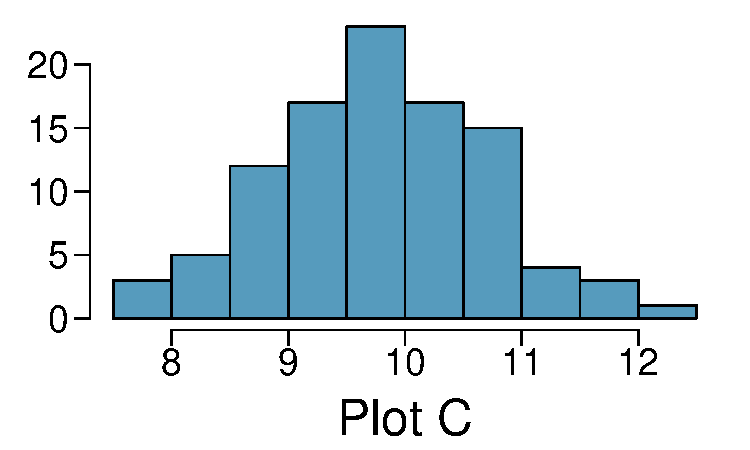
\includegraphics[width=0.32\textwidth]{4-4_clt/figures/cltSimRS/cltSimRS_n49}

\end{frame}

%%%%%%%%%%%%%%%%%%%%%%%%%%%%%%%%%%%%